% ============================================================
\chapter{予想の当たり具合から $\Omega$ を決める}\label{ch:accuracy}

ここまでの方法（He--Litterman、Meucci、Idzorek）は、$\Omega$ を何かとの比で決めていた。この章では、$\Omega$ を予想の当たり具合から決める。過去の予想と実際の結果の記録があれば、「どれだけ信じてよいか」はデータで答えられる。

中心になる結果は次のとおりである。Meucci の市場版の BL で、ビューの不確かさを $\omega=\sigma^2(1/\IC^2-1)$ と置くと、事後の期待リターンは Grinold の式 $\alpha=\IC\cdot\sigma\cdot z$ とちょうど一致する。運用の実務で昔から使われている「予想を当たり具合で縮める」式と、BL は同じものだということである。

\section{当たり具合を測る 3 つの量}

予想 $q_i$ と、その後に実現したリターン $r_i$ の組（銘柄 $i=1,\dots,N$、時点 $t=1,\dots,T$）があるとする。当たり具合の測り方は 3 つある。

\begin{description}[leftmargin=2em,style=nextline]
\item[情報係数（IC）] 予想と実際の相関 $\IC=\mathrm{corr}(q,r)$。順位相関で測ることも多い。大きさの単位によらない。
\item[較正の傾き $b$] 実際を予想に回帰したときの傾き $b=\Cov(q,r)/\Var(q)$。予想の大きさまで含めた当たり具合で、$b=\IC\cdot\sigma_r/\sigma_q$ の関係がある。
\item[誤差の 2 乗の平均（MSE）] $\E[(q-r)^2]$。予想の外れの大きさそのもの。
\end{description}

$b=1$ なら、予想の大きさはちょうどよい。$b<1$ なら予想は大きすぎ（自信過剰）、$b>1$ なら小さすぎ（控えめすぎ）、$b<0$ なら向きが逆である。BL に入れるときに必要なのは、この 3 つのうち $b$（または IC と、予想と実際の散らばりの比）である。

\section{Grinold の式}

Grinold（1994）は、予想の点数を期待リターンに直す式として、
\begin{equation}
\alpha_i=\IC\cdot\sigma_i\cdot z_i
\label{eq:grinold}
\end{equation}
を示した（論文の題名は \textit{Alpha is Volatility Times IC Times Score}）。$z_i$ は銘柄 $i$ の点数を平均 0、標準偏差 1 にそろえたもの、$\sigma_i$ はその銘柄のリターンの標準偏差（ここでは特異リスクに限らず、予想する期間のリターンの標準偏差とする）、$\alpha_i$ は期待リターンの、市場の見込みからのずれである。

この式は、予想 $q$ と実際 $r$ が 2 変量正規分布に従うときの条件付き期待値そのものである。
\begin{equation}
\E[r\mid q]=\E[r]+\mathrm{corr}(q,r)\,\sigma_r\,\frac{q-\E[q]}{\sigma_q}=\E[r]+\IC\cdot\sigma_r\cdot z
\end{equation}
つまり Grinold の式は、「予想を見たあとで、実現するリターンの平均はどうなるか」を、回帰で答えたものである。予想がほとんど当たらないなら（IC が小さいなら）、期待リターンはほとんど動かない。

IC は、優れた運用者でも 0.05 前後とされる。月次の標準偏差が 8\% の銘柄なら、点数が 1 標準偏差高い銘柄の期待リターンは $0.05\times8\%=0.4\%$ しか上がらない。

\section{市場版の BL と Grinold の式は同じ}\label{sec:grinold-bl}

市場版の BL（\chapref{ch:hlmeucci}）で、1 資産・1 ビューの場合を考える。来期のリターン $x$ は $\mathcal N(\pi,\sigma^2)$ に従い、ビュー $v$ は $x$ に外れ $\varepsilon\sim\mathcal N(0,\omega)$ が乗ったもの、つまり $v=x+\varepsilon$ とする。事後の期待値は、式~\eqref{eq:mbl-mu} から
\begin{equation}
\E[x\mid v]=\pi+\frac{\sigma^2}{\sigma^2+\omega}(v-\pi)
\label{eq:mbl-scalar}
\end{equation}
である。この設定で予想 $v$ と実際 $x$ の相関を計算すると、$\Cov(v,x)=\sigma^2$、$\Var(v)=\sigma^2+\omega$ なので、
\begin{equation}
\IC=\mathrm{corr}(v,x)=\frac{\sigma}{\sqrt{\sigma^2+\omega}},\qquad
\IC^2=\frac{\sigma^2}{\sigma^2+\omega}
\end{equation}
となる。式~\eqref{eq:mbl-scalar} の採用率は、ちょうど $\IC^2$ である。逆に解くと
\begin{equation}
\boxed{\;\omega=\sigma^2\Bigl(\frac{1}{\IC^2}-1\Bigr)\;}
\label{eq:omega-ic}
\end{equation}
である。さらに、予想を標準化した点数 $z=(v-\pi)/\sqrt{\sigma^2+\omega}=(v-\pi)\,\IC/\sigma$ を使うと、
\begin{equation}
\E[x\mid v]-\pi=\IC^2\,(v-\pi)=\IC^2\cdot\frac{\sigma z}{\IC}=\IC\cdot\sigma\cdot z
\end{equation}
となり、Grinold の式~\eqref{eq:grinold} と一致する。

\begin{thmbox}[市場版の BL と Grinold の式]
予想の外れの分散を $\omega=\sigma^2(1/\IC^2-1)$ と置いた市場版の BL の事後の期待リターンは、Grinold の式 $\pi+\IC\cdot\sigma\cdot z$ に等しい。このときの採用率は $\IC^2$ である。
\end{thmbox}

\begin{table}[htbp]
\centering
\caption{IC と、それに見合う採用率・$\omega$。「生の予想の広がり」は、$v=x+\varepsilon$ の設定で予想の標準偏差が実際の何倍か。右端は、月次の標準偏差 8\% の銘柄で、点数が 1 標準偏差高いときの期待リターンの上乗せ（月次 \%）。}
\label{tab:ic}
\tabin{ic}
\end{table}

\tabref{tab:ic} のとおり、IC が 0.05 なら採用率は 0.25\%、$\omega$ は $\sigma^2$ の 399 倍である。He--Litterman の採用率 50\% は IC で言えば 0.71 に当たる。来月のリターンを予想して IC が 0.7 になることは、まずない。

\subsection*{シミュレーションで確かめる}

$v=x+\varepsilon$ の設定で、IC が 0.10 になるように \V{sim.n} 組の $(x,v)$ を作った（\figref{fig:ic-sim}）。実際の IC は \V{sim.ic} である。

\begin{figure}[htbp]
\centering
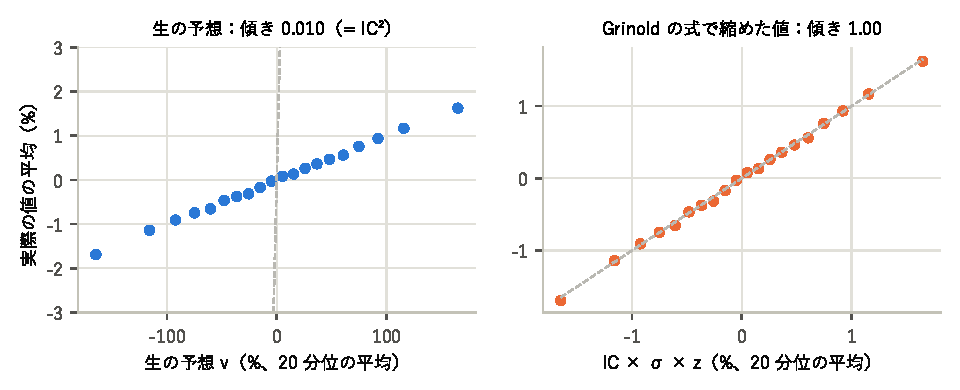
\includegraphics[width=0.95\linewidth]{fig_ic_sim.pdf}
\caption{予想の 20 分位ごとの、実際の値の平均。左：生の予想 $v$ は、実際の値に対して大きすぎる（傾き $\approx\IC^2$）。右：Grinold の式で縮めた値は、実際の値と傾き 1 で並ぶ。破線は 45 度の線。}
\label{fig:ic-sim}
\end{figure}

生の予想 $v$ に対する実際の値の傾きは \V{sim.slope.raw} で、$\IC^2=0.01$ に一致する。生の予想を期待リターンとしてそのまま使うと、100 倍の自信過剰になる。Grinold の式で縮めた値の傾きは \V{sim.slope.post} で、ほぼ 1 である。BL の言葉で言えば、正しい採用率で混ぜると、予想は「較正された」状態になる。

\section{元の BL に直す}

元の BL（$\tau$ を使う形）で同じ採用率にするには、$\tau\sigma^2/(\tau\sigma^2+\omega)=\IC^2$ から
\begin{equation}
\omega=\tau\sigma^2\Bigl(\frac{1}{\IC^2}-1\Bigr)
\label{eq:omega-ic-tau}
\end{equation}
と置けばよい。Idzorek の確信度で言えば $C=\IC^2$ である。この $\omega$ は $\tau$ に比例するので、$\tau$ は消える。

ここで注意が 1 つある。式~\eqref{eq:omega-ic} と式~\eqref{eq:omega-ic-tau} は、1 資産・1 ビューで採用率を合わせたものである。ビューが多く、$\Omega$ を対角にすると、ビューの相関を通じて採用率が変わる（\secref{sec:diag-trap}）。複数のビューで「どの銘柄も同じ割合 $s$ だけ動かす」には、$\Omega$ を $\Sigma$ に比例させる。
\begin{equation}
\Omega=\tau\Bigl(\frac1s-1\Bigr)P\Sigma P\T\quad\Longrightarrow\quad
\muBL=\Pi+s\,\Sigma P\T(P\Sigma P\T)^{-1}(Q-P\Pi)
\label{eq:omega-prop}
\end{equation}
$P=I$（すべての銘柄に絶対ビュー）なら $\muBL=\Pi+s(Q-\Pi)$ で、すべての銘柄が同じ割合だけビューへ動く。

\section{較正の傾きで測る}\label{sec:slope}

実際には、IC と予想の大きさ（予想の標準偏差）は別々にずれる。LLM の予想のように、予想の散らばりが実際の散らばりと無関係に決まっている場合、IC だけで縮めても大きさが合わない。このときは、較正の傾き $b$ を直接測り、それを採用率にするのが簡単である。

\begin{enumerate}
\item 時点ごとに、予想 $q_{it}$ と実際 $r_{it}$ から、その時点の平均を引く（全体の水準の当たり外れを除き、銘柄間の差だけを見る）。
\item すべての時点をまとめて、実際を予想に回帰した傾き $b=\sum_{i,t}\tilde q_{it}\tilde r_{it}\big/\sum_{i,t}\tilde q_{it}^2$ を求める（$\tilde{}$ は平均を引いたもの）。
\item 判断日より前の時点だけで $b$ を計算する（先読みしない）。データがないうちは $b=0$（均衡のまま）とする。
\item $b$ を 0 から 1 の範囲に収め、式~\eqref{eq:omega-prop} の $s$ として使う。$b\le0$ なら、ビューは使わない。
\end{enumerate}

本プロジェクトの LLM の予想で計算すると、月ごとの傾きの平均は \V{llm.slope.mean}（$t$ 値 \V{llm.slope.t}）、30 か月をまとめた傾きは \V{llm.slope.pooled} だった（\chapref{ch:project}）。予想の散らばりのうち、実際の差につながっているのは 7\% 程度で、残りは雑音である。

\subsection*{推定の誤差}

$b$ や IC も推定値なので、誤差がある。月ごとの横断面の IC は、月によって大きくぶれる。本プロジェクトでは、月ごとの順位相関の平均が \V{llm.ic.mean}、$t$ 値が \V{llm.ic.t} だった。この $t$ 値から逆算すると、月ごとの IC の標準偏差は 0.19 程度で、平均 0.05 を $t$ 値 2 で確かめるには約 55 か月分のデータが要る。

推定値が不確かなときは、推定値をそのまま使うより、0 に寄せて使うほうが安全である。例えば、傾きの推定値 $\hat b$ と、その標準誤差 $\mathrm{se}$ から、$\hat b\cdot\max\{0,1-\mathrm{se}^2/\hat b^2\}$ のように縮める（$t$ 値が小さいほど 0 に近づく）。この資料の計算（\chapref{ch:project}）では、簡単のため縮めずに使ったが、データが少ない時期は $b$ が 0 になる月が多かった（30 か月のうち \V{bt.b.zero} か月）。

\section{誤差の分散から測る（元の BL）}

元の BL で、ビューが期待リターン $\mu$ についてのものだとすると、ビューの外れの分散 $\omega$ は「$Q$ と $\mu$ の差」の分散である。しかし $\mu$ は見えない。見えるのは実現したリターンの平均 $\bar r$ で、$\bar r=\mu+\eta$、$\eta$ の分散は $\sigma^2/n$（$n$ は平均した日数）である。$Q$ の外れと $\eta$ が独立なら、
\begin{equation}
\E[(Q-\bar r)^2]=\omega+\frac{\sigma^2}{n}
\quad\Longrightarrow\quad
\hat\omega=\overline{(Q-\bar r)^2}-\overline{\sigma^2/n}
\label{eq:omega-err}
\end{equation}
で $\omega$ を推定できる。右辺の第 2 項は、たとえ $\mu$ を完全に知っていても避けられない外れである。

\begin{exbox}[本プロジェクトのデータ]
LLM の予想（翌月の日次の平均リターン）について、30 か月の平均で計算すると、誤差の 2 乗の平均は \V{llm.mse}、避けられない外れ $\sigma^2/n$ の平均は \V{llm.noise} だった。差の $\hat\omega$ は約 $1.6\times10^{-5}$ で、標準偏差に直すと 1 日あたり 0.4\% 程度である。一方、LLM の回答の分散の平均は \V{llm.om.mean} で、$\hat\omega$ の 5 分の 1 以下だった。回答の分散を $\Omega$ にすると、外れを 5 分の 1 以下に見積もることになる。
\end{exbox}

この方法の弱点は、引き算をするので推定が不安定なことである。避けられない外れが大きいと、差が負になることもある。そのときは、予想は「平均を知らないのと同じくらい」しか当たっていない、という意味で、ビューを使わないのが正しい。

\section{基本法則とビューの数}

Grinold と Kahn の「アクティブ運用の基本法則」は、事前の情報レシオを
\begin{equation}
\IR\approx\IC\sqrt{\mathrm{BR}}
\end{equation}
と近似する。BR（breadth）は、1 年あたりの独立な予想の数である。IC が小さくても、独立な予想がたくさんあれば、情報レシオは大きくなる。500 銘柄を毎月予想するなら $\mathrm{BR}=6000$、$\IC=0.05$ で $\IR\approx3.9$ という計算になる。

この計算は「予想の外れが銘柄ごと・月ごとに独立」という仮定に強く依存する。実際には、同じ情報源から作った予想の外れは相関し、独立な予想の数ははるかに少ない。BL で $\Omega$ を対角にすると、まさにこの仮定を置いたことになり、ビューの数だけ確信が積み上がる（\secref{sec:diag-trap}）。事前の情報レシオが 1 を大きく超えたら、独立の仮定を疑うのがよい。

\begin{tipbox}[コツ：当たり具合から $\Omega$ を決める]
\begin{enumerate}
\item 予想と実際の記録を残す。それが $\Omega$ を決める唯一の確かな材料である。
\item 採用率は、較正の傾き $b$（または $\IC^2$）にする。市場版なら $\omega=\sigma^2(1/\IC^2-1)$、元の BL なら $\omega=\tau\sigma^2(1/\IC^2-1)$。
\item ビューが多いときは、$\Omega$ を $P\Sigma P\T$ に比例させ、どのビューも同じ割合で動かす。対角にしない。
\item 傾きは判断日より前のデータだけで測り、データが少ないうちは 0 に寄せる。
\item 事前の情報レシオが 1 を大きく超えたら、確信を積み上げすぎていないか確かめる。
\end{enumerate}
\end{tipbox}

\begin{keybox}[この章のまとめ]
\begin{itemize}
\item 当たり具合は、IC、較正の傾き $b$、誤差の 2 乗の平均で測れる。BL に必要なのは $b$（または $\IC^2$）である。
\item 市場版の BL で $\omega=\sigma^2(1/\IC^2-1)$ と置くと、Grinold の式 $\IC\cdot\sigma\cdot z$ と一致し、採用率は $\IC^2$ になる。IC が 0.05 なら 0.25\% である。
\item 元の BL では、誤差の 2 乗の平均から、避けられない外れ $\sigma^2/n$ を引いた値が $\omega$ の推定値になる。
\item 基本法則 $\IR\approx\IC\sqrt{\mathrm{BR}}$ も、対角の $\Omega$ も、外れが独立という仮定に頼っている。
\end{itemize}
\end{keybox}
